\subsection{2.4. Mô hình hóa luồng hoạt động và quy trình nghiệp vụ}
Để làm rõ trình tự điều khiển, các nút quyết định rẽ nhánh (\textit{Decision/Merge Nodes}) và cơ chế phối hợp thông điệp giữa các tác nhân trong những luồng nghiệp vụ phức tạp nhất của hệ thống 5Share, nhóm thực hiện mô hình hóa 02 biểu đồ hoạt động (\textit{Activity Diagram} chuẩn UML 2.5) và 01 biểu đồ quy trình nghiệp vụ cộng tác (\textit{Collaboration Diagram} chuẩn OMG BPMN 2.0).

\subsubsection{2.4.1. Biểu đồ hoạt động luồng đóng góp và kiểm tra trùng lặp tự động}
Biểu đồ hoạt động thứ nhất (Hình~\ref{fig:ad1}) mô tả chi tiết luồng kết hợp giữa các ca sử dụng \texttt{UC07} (Đóng góp tài liệu), \texttt{UC08} (Kiểm tra tài liệu trùng lặp) và \texttt{UC11} (Theo dõi trạng thái tài liệu) qua 02 làn bơi (\textit{Swimlanes}): Làn Sinh viên và Làn Hệ thống 5Share.

\begin{figure}[H]
\centering
\IfFileExists{chuong2/images/ad1_dong_gop_kiem_tra_trung.png}{%
    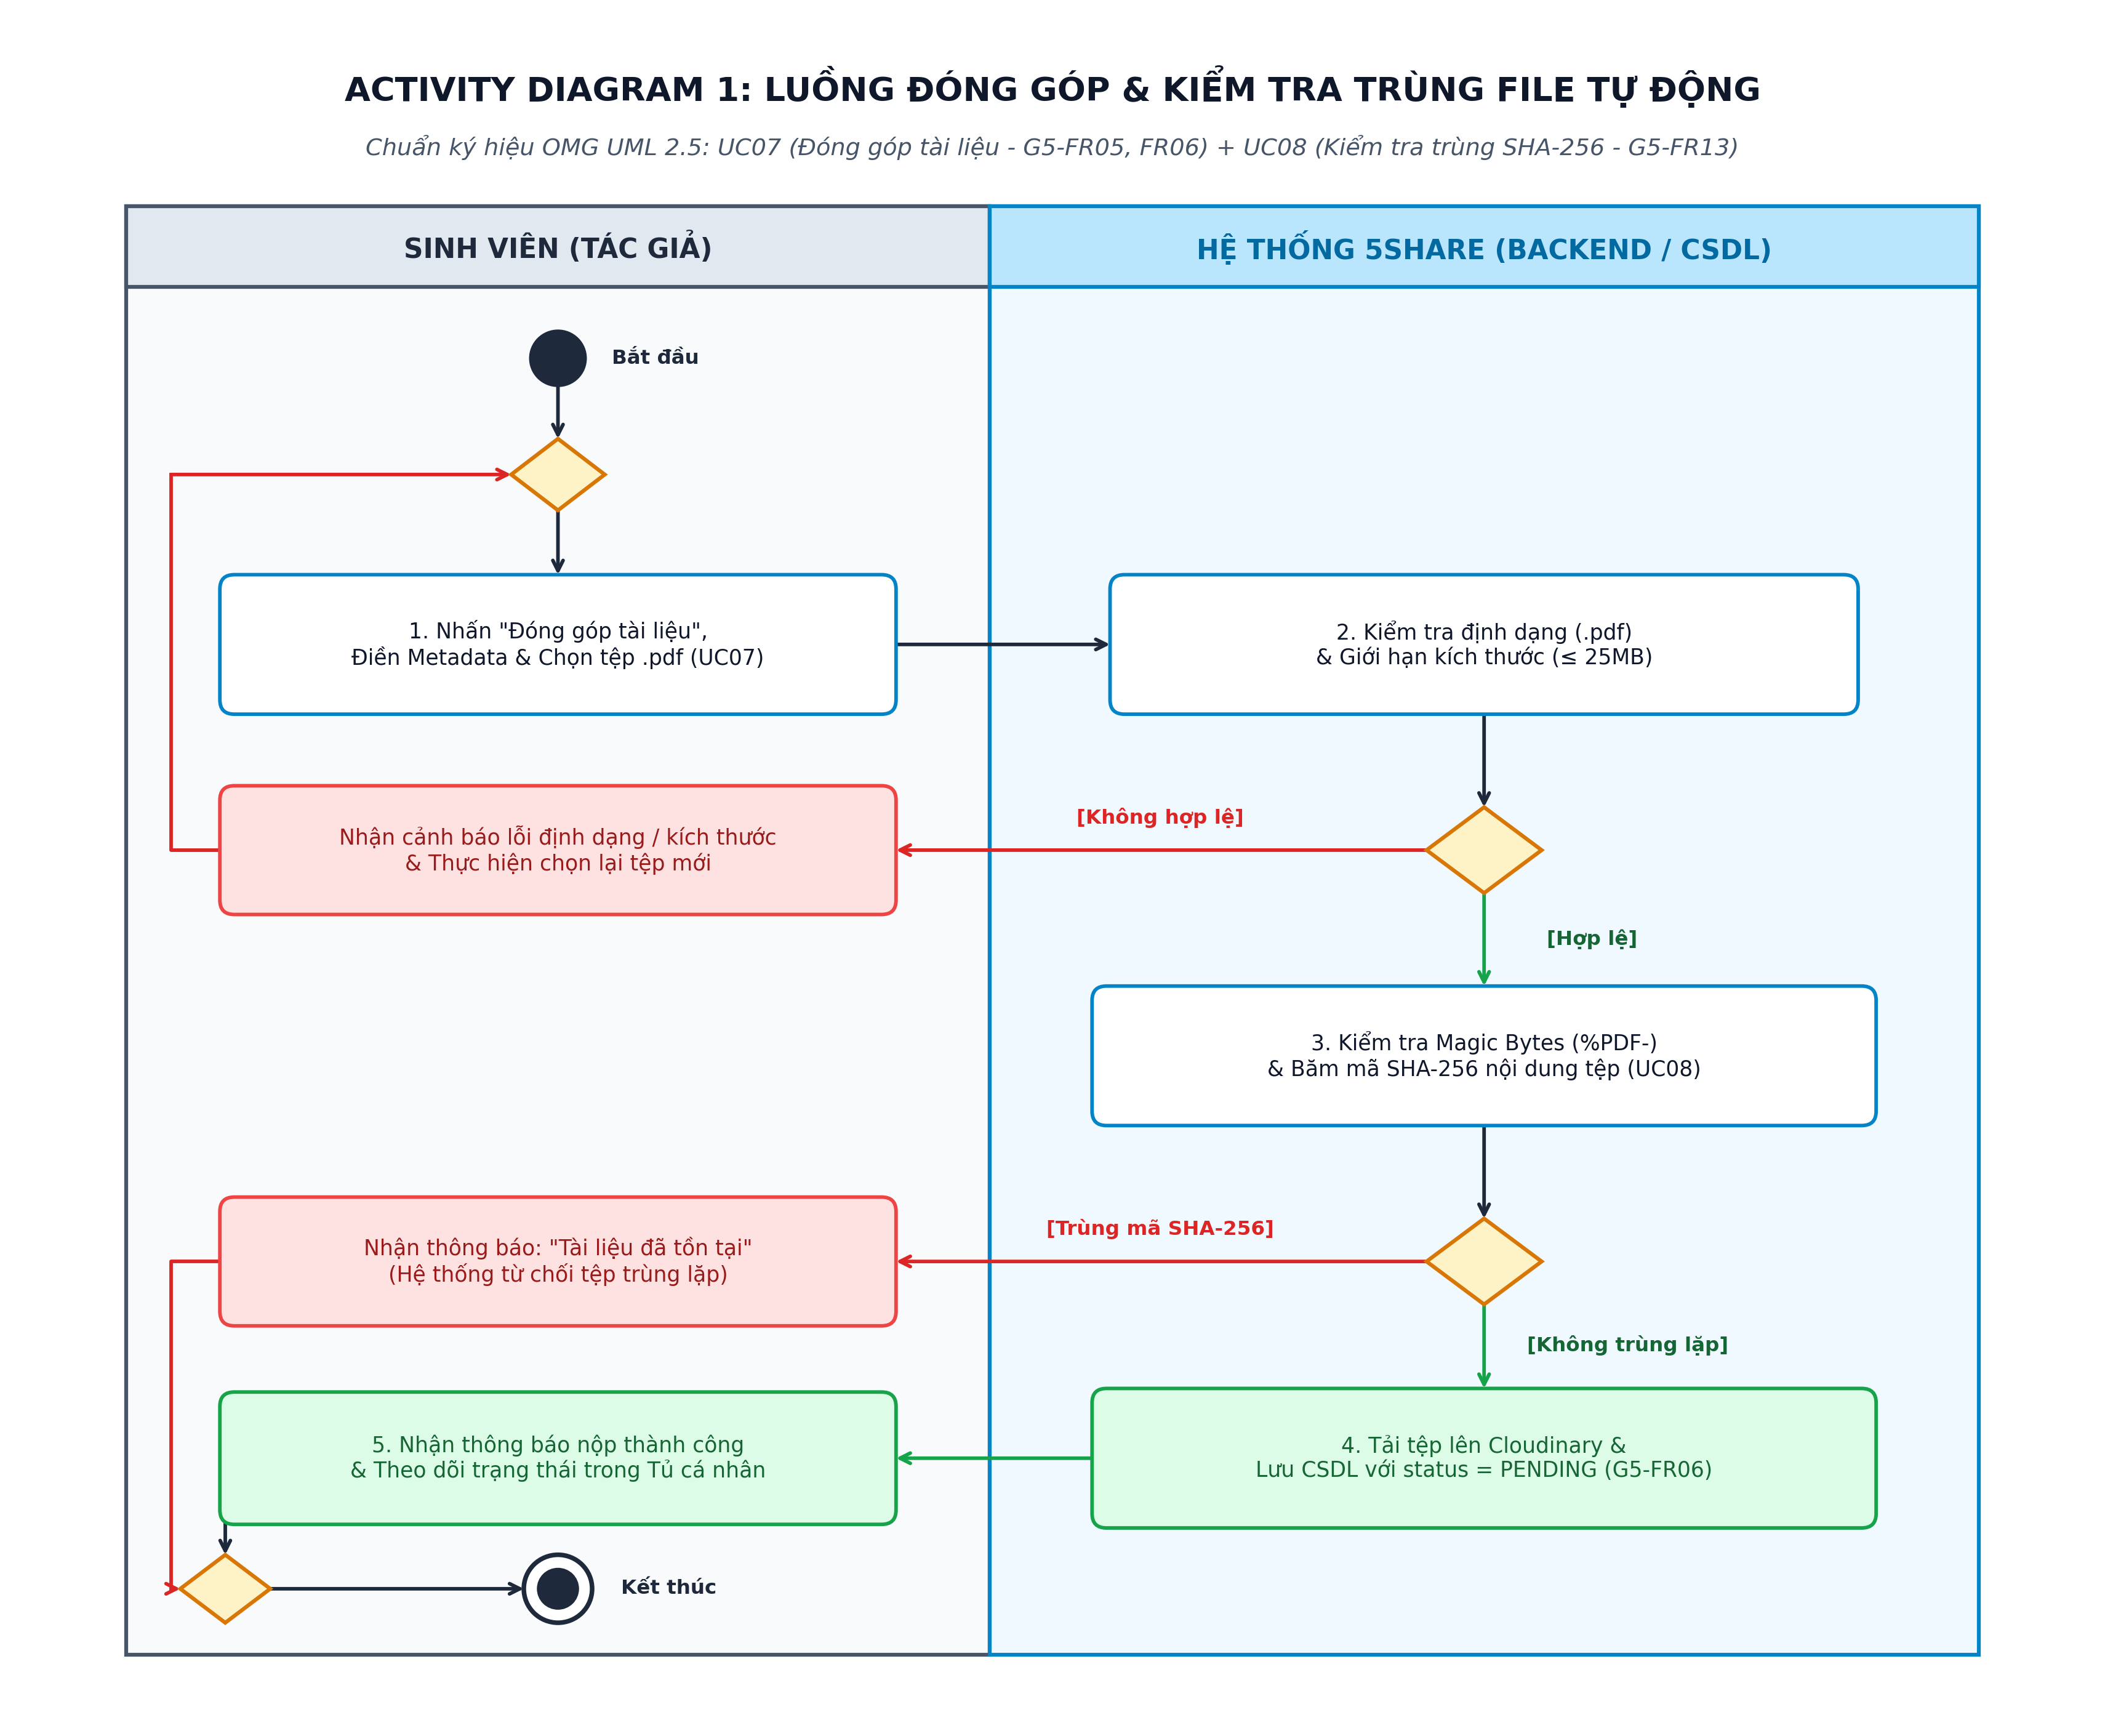
\includegraphics[width=0.96\textwidth]{chuong2/images/ad1_dong_gop_kiem_tra_trung.png}%
}{%
    \fbox{\parbox{0.95\textwidth}{\centering \vspace{3cm}\textbf{[Hình 2.3: Biểu đồ hoạt động luồng đóng góp và kiểm tra trùng lặp tự động (AD1)]}\vspace{3cm}}}%
}
\caption{Biểu đồ hoạt động luồng đóng góp và kiểm tra trùng lặp tự động (AD1)}
\label{fig:ad1}
\end{figure}

Quy trình kiểm soát tự động trên biểu đồ diễn ra theo 3 chốt chặn kỹ thuật liên tiếp:
\begin{itemize}[leftmargin=*,noitemsep]
    \item \textbf{Chốt chặn 1 -- Kiểm tra biểu mẫu Metadata:} Sau khi sinh viên chọn tệp PDF và nhập đầy đủ các trường Metadata bắt buộc (Tên tài liệu, Môn học, Loại học liệu, Mô tả), hệ thống kiểm tra tính hợp lệ của biểu mẫu. Nếu thiếu thông tin, luồng điều khiển đi qua nút gộp (\textit{Merge Node}) quay lại bước nhập liệu để sinh viên bổ sung.
    \item \textbf{Chốt chặn 2 -- Kiểm tra định dạng và dung lượng:} Hệ thống kiểm tra định dạng tệp (\texttt{.pdf}), chữ ký nhị phân đầu tệp (Magic Bytes \texttt{\%PDF-}) và giới hạn dung lượng $\le$ 25MB. Nếu tệp tin vượt quá dung lượng hoặc giả mạo định dạng, hệ thống cảnh báo lỗi và yêu cầu chọn lại tệp.
    \item \textbf{Chốt chặn 3 -- Băm SHA-256 chống trùng lặp:} Hệ thống kích hoạt thuật toán băm \texttt{SHA-256} trên nội dung nhị phân của tệp tin (\texttt{UC08}) và đối chiếu với cột \texttt{file\_hash} trong bảng \texttt{documents}. Nếu mã băm đã tồn tại, hệ thống từ chối tiếp nhận và kết thúc luồng tại nút kết thúc (\textit{Activity Final Node}). Nếu mã băm là duy nhất, hệ thống tải tệp lên dịch vụ đám mây Cloudinary, khởi tạo bản ghi với trạng thái \texttt{status = 'PENDING'} và chuyển sang màn hình theo dõi trạng thái tài liệu (\texttt{UC11}).
\end{itemize}

\subsubsection{2.4.2. Biểu đồ hoạt động luồng tra cứu, xem trước và tải học liệu}
Biểu đồ hoạt động thứ hai (Hình~\ref{fig:ad2}) mô tả luồng nghiệp vụ kết hợp giữa các ca sử dụng \texttt{UC05} (Tìm kiếm và lọc tài liệu), \texttt{UC06} (Xem trước tài liệu), \texttt{UC12} (Tải tài liệu về máy) và \texttt{UC01} (Đăng nhập hệ thống) giữa 02 làn bơi: Người dùng (Khách vãng lai / Sinh viên) và Hệ thống 5Share.

\begin{figure}[H]
\centering
\IfFileExists{chuong2/images/ad2_tra_cuu_preview_tai_ve.png}{%
    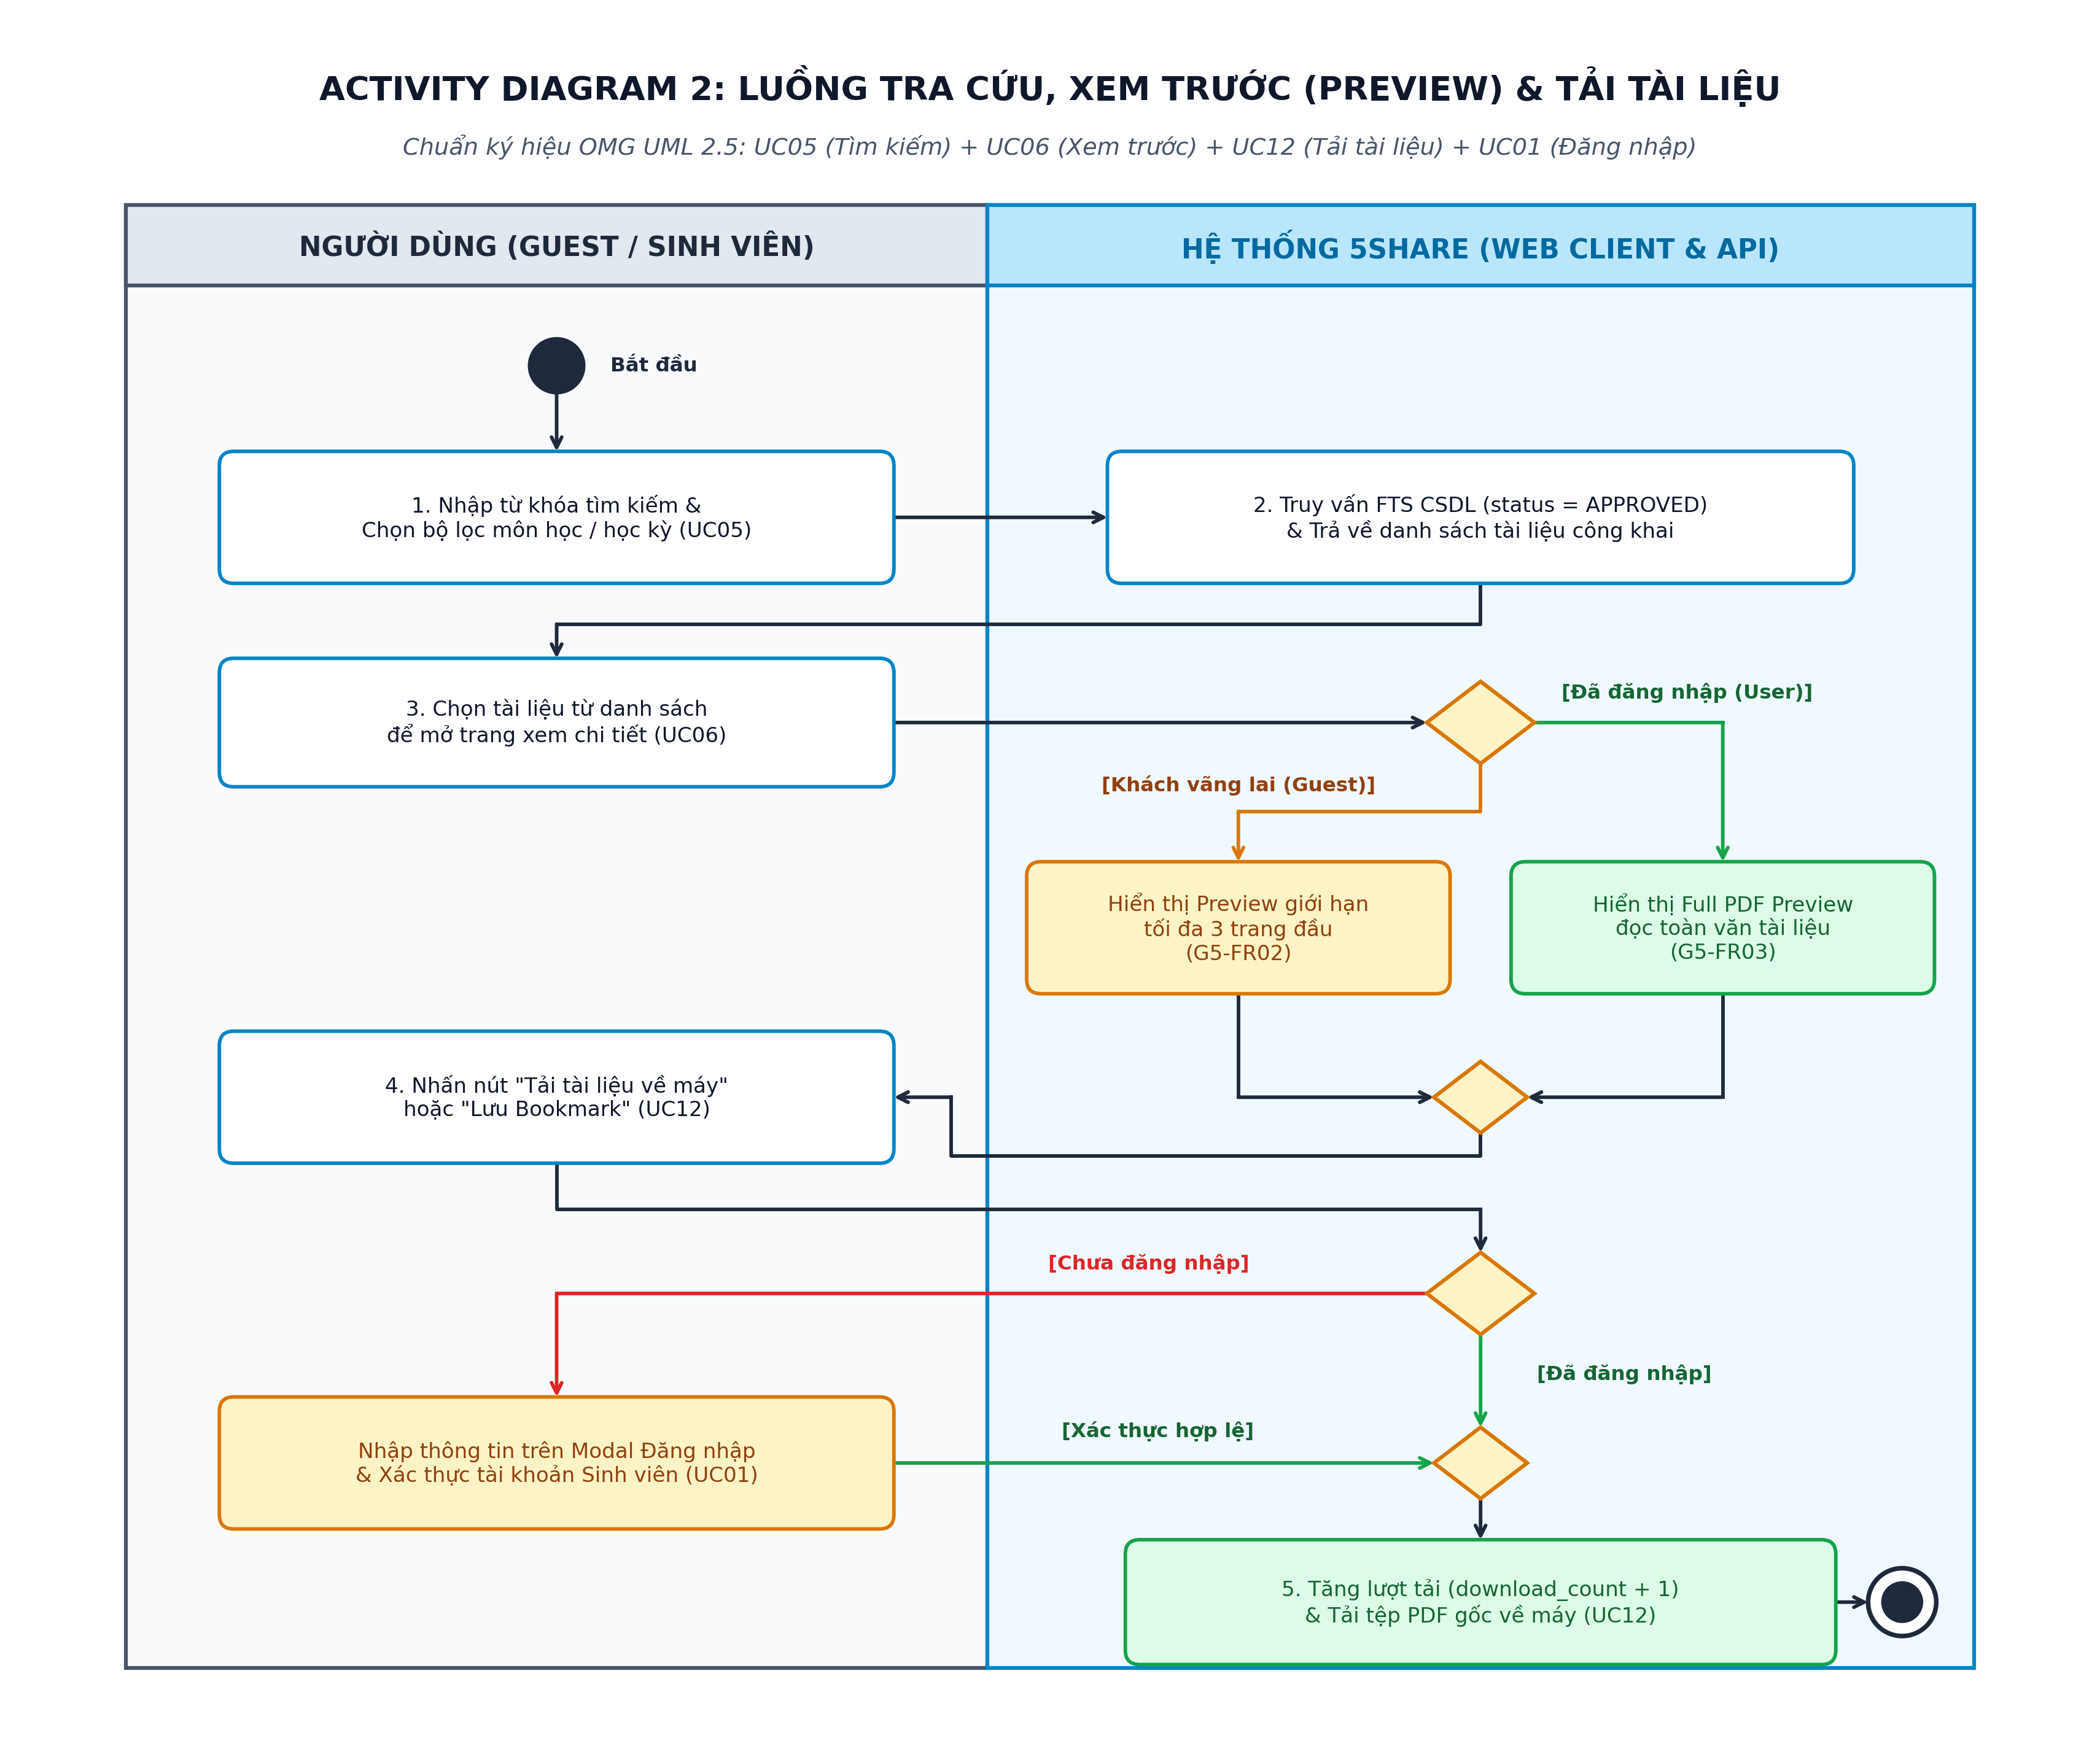
\includegraphics[width=0.96\textwidth]{chuong2/images/ad2_tra_cuu_preview_tai_ve.png}%
}{%
    \fbox{\parbox{0.95\textwidth}{\centering \vspace{3cm}\textbf{[Hình 2.4: Biểu đồ hoạt động luồng tra cứu, xem trước và tải học liệu (AD2)]}\vspace{3cm}}}%
}
\caption{Biểu đồ hoạt động luồng tra cứu, xem trước và tải học liệu (AD2)}
\label{fig:ad2}
\end{figure}

Luồng hoạt động thể hiện rõ cơ chế phân quyền truy cập tài nguyên theo trạng thái xác thực:
\begin{itemize}[leftmargin=*,noitemsep]
    \item \textbf{Giai đoạn tra cứu và lọc:} Người dùng nhập từ khóa hoặc chọn bộ lọc theo môn học, loại học liệu. Hệ thống truy vấn cơ sở dữ liệu bằng Full-Text Search đối với các bản ghi có \texttt{status = 'APPROVED'}. Nếu không có kết quả khớp, hệ thống thông báo để người dùng điều chỉnh từ khóa.
    \item \textbf{Giai đoạn xem trước trực tuyến (Preview):} Khi người dùng chọn một học liệu, hệ thống hiển thị bản xem trước trực tuyến trên trình duyệt (\texttt{UC06}). Khách vãng lai được đọc thử tối đa 3 trang đầu tiên; nếu chỉ dừng lại ở việc xem thử và đóng trang, luồng hoạt động kết thúc bình thường.
    \item \textbf{Giai đoạn kiểm tra phiên đăng nhập và tải tệp gốc:} Khi người dùng nhấn nút ``Tải xuống tệp gốc (.pdf)'' (\texttt{UC12}), hệ thống kiểm tra mã phiên xác thực JWT. Nếu người dùng đã đăng nhập, hệ thống tăng bộ đếm \texttt{download\_count} thêm 1 và trả luồng tệp PDF gốc về thiết bị. Nếu người dùng là Khách vãng lai, hệ thống mở cửa sổ yêu cầu đăng nhập (\texttt{UC01}); ngay sau khi xác thực thành công, luồng điều khiển hợp nhất tại nút Merge để tự động thực thi việc tải tệp mà không bắt người dùng phải tìm kiếm lại từ đầu.
\end{itemize}

\subsubsection{2.4.3. Biểu đồ quy trình nghiệp vụ (BPMN 2.0) vòng đời kiểm duyệt và khai thác học liệu}
Để mô tả toàn diện sự phối hợp liên tác nhân xuyên suốt vòng đời của một học liệu số từ lúc sinh viên đóng góp, trải qua kiểm duyệt hai tầng cho đến khi xuất bản công khai hoặc bị thu hồi do vi phạm, biểu đồ quy trình nghiệp vụ cộng tác theo chuẩn OMG BPMN 2.0 gồm 03 bể (\textit{Pools}) độc lập được xây dựng tại Hình~\ref{fig:bpmn_vong_doi}:

\begin{figure}[H]
\centering
\IfFileExists{chuong2/images/bpmn_vong_doi_tai_lieu.png}{%
    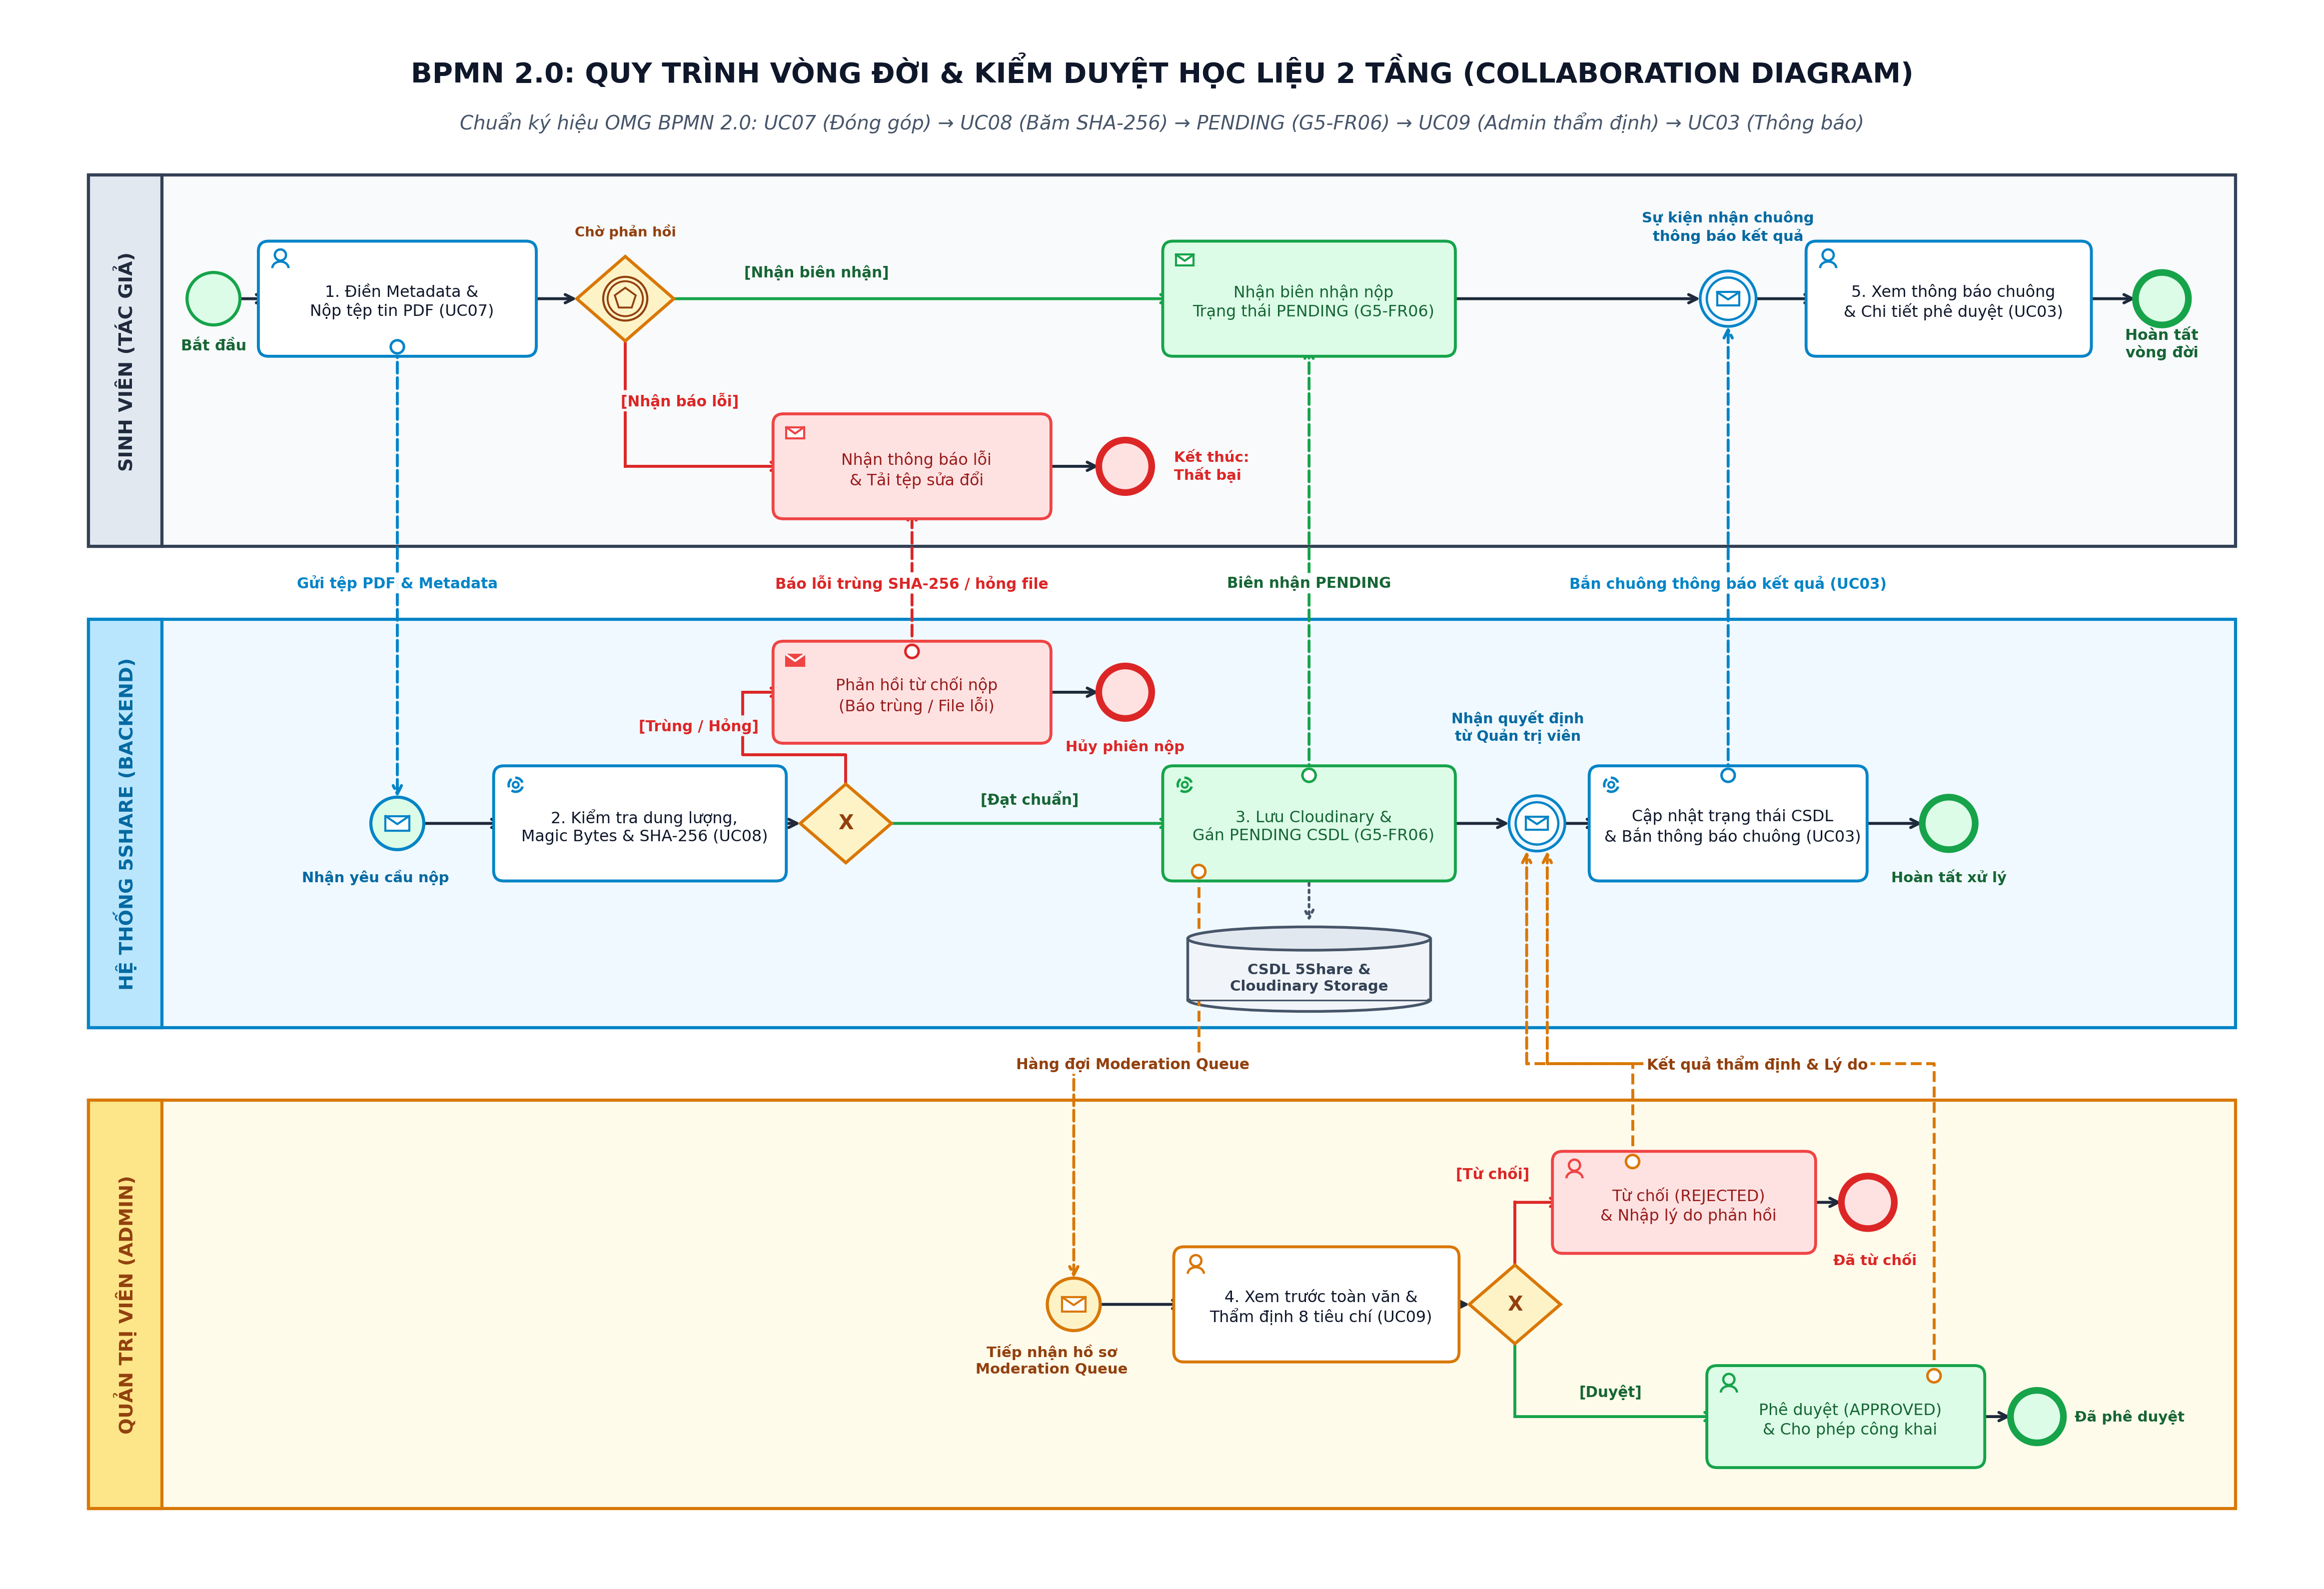
\includegraphics[width=0.99\textwidth]{chuong2/images/bpmn_vong_doi_tai_lieu.png}%
}{%
    \fbox{\parbox{0.95\textwidth}{\centering \vspace{3cm}\textbf{[Hình 2.5: Biểu đồ quy trình nghiệp vụ (BPMN 2.0) vòng đời kiểm duyệt và khai thác học liệu trên 5Share]}\vspace{3cm}}}%
}
\caption{Biểu đồ quy trình nghiệp vụ (BPMN 2.0) vòng đời kiểm duyệt và khai thác học liệu trên 5Share}
\label{fig:bpmn_vong_doi}
\end{figure}

Cấu trúc biểu đồ tuân thủ nghiêm ngặt các nguyên tắc ký hiệu của chuẩn OMG BPMN 2.0:
\begin{itemize}[leftmargin=*,noitemsep]
    \item \textbf{Phân tách bể (Pools) và làn (Lanes):} Biểu đồ phân tách rõ 03 Pool đại diện cho 3 chủ thể: (1) Pool Sinh viên (Tác giả đóng góp \& Người học khai thác); (2) Pool Hệ thống 5Share (chứa 2 làn nội bộ: Làn Kiểm tra tự động \& Xử lý sự kiện, và Làn Lưu trữ đám mây \& Cơ sở dữ liệu); (3) Pool Quản trị viên (Ban kiểm duyệt học liệu).
    \item \textbf{Luồng tuần tự (Sequence Flow) và Luồng thông điệp (Message Flow):} Mọi tương tác bên trong cùng một Pool được nối bằng mũi tên nét liền (\textit{Sequence Flow}). Mọi tương tác vượt qua ranh giới giữa hai Pool khác nhau bắt buộc sử dụng đường nét đứt có vòng tròn ở gốc (\textit{Message Flow}), kết nối từ các tác vụ gửi (\textit{Send Task}) hoặc tác vụ dịch vụ (\textit{Service Task}) đến các sự kiện bắt thông điệp (\textit{Message Start/Intermediate Catch Event}).
    \item \textbf{Cổng hướng sự kiện (Event-Based Gateway) và Vòng đời hậu kiểm:} Sau khi gửi biểu mẫu đóng góp (\texttt{UC07}), luồng của Sinh viên đi vào cổng rẽ nhánh dựa trên sự kiện (\textit{Event-Based Gateway}) để chờ phản hồi từ hệ thống qua 3 nhánh sự kiện bắt thông điệp: (1) Nhận cảnh báo lỗi kỹ thuật hoặc trùng mã băm \texttt{SHA-256} (từ \texttt{UC08}); (2) Nhận thông báo tài liệu bị từ chối kèm lý do (\texttt{REJECTED}); (3) Nhận thông báo tài liệu được phê duyệt (\texttt{APPROVED}) và cộng điểm đóng góp. Đối với tài liệu đã xuất bản, nếu bị sinh viên khác gửi báo cáo vi phạm (\texttt{UC04}) và Quản trị viên xác nhận vi phạm nặng (\texttt{UC09}), hệ thống thực thi tác vụ thu hồi (\texttt{status = 'HIDDEN'} / \texttt{'DELETED'}) để bảo đảm độ tinh sạch của kho học liệu.
\end{itemize}
